%!TEX root = ../thesis.tex
\newchap{Signal reconstruction and interpretation}\label{sec:kin}
\vspace{-1cm}
\minitoc
\vspace{0.5cm}
This chapter focuses on the kinematical reconstruction and interpretation of the signal events tackling the jet-parton assignment problem.
\\
\TODO{Reintroduci il ranking (cerca su git se salvato)}
\\
The jet-parton assignment is first done with just one jet, the one b-jet associated with the decay of the top quark that decays into the W boson that decays leptonically. This simplified benchmark is used to perform a feature ranking exploiting the $N+1,\: N-1$ method and to select the best model that will be used in the full jet-paron assignment.

\begin{minipage}[H]{\linewidth}
\begin{minipage}{0.35\linewidth}
        \centering
        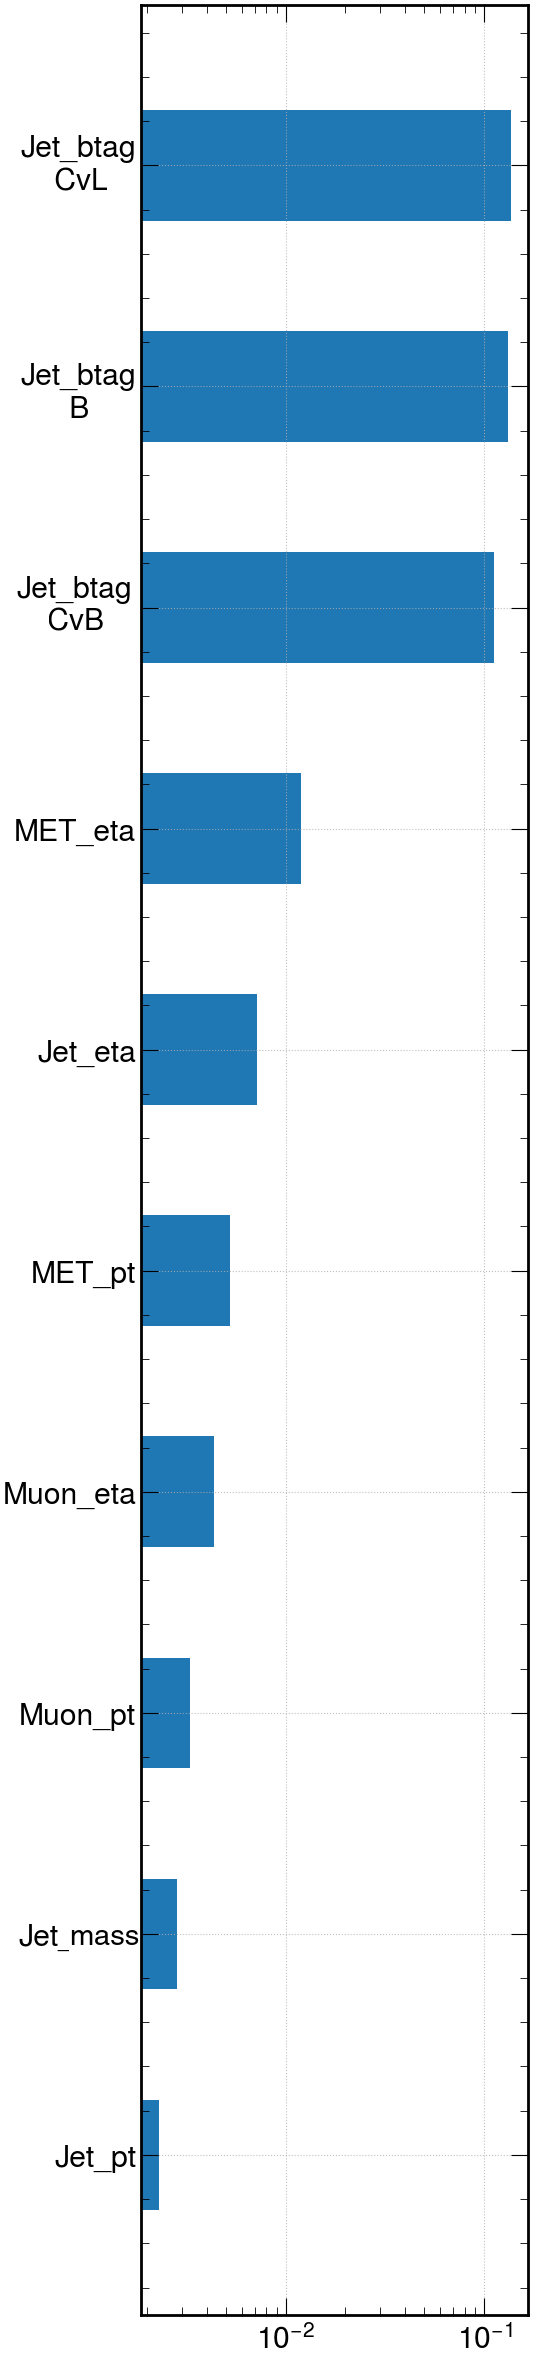
\includegraphics[height=0.92\textheight]{fig//chap08-kin_reco/ranking1D.png}
        \captionof{figure}{Unidimensional feature ranking using the metric $d$ between flattened signal observables and \ttbar semileptonic observables }
        \label{fig:1Drank}
\end{minipage}
\hfill
\begin{minipage}{0.62\linewidth}
\section{Unidimensional feature ranking}
The simplest way to select relevant features that can discriminate the signal from the background is to look at the distribution of different observables, selecting the ones with the most different shapes.\\
The "shape difference" between two histograms can be quantified by the following metric

\begin{equation}
    d=\frac{1}{2}\sum_b \bigg| y_b^{(1)}-y_b^{(2)} \bigg|
\end{equation}
where $y_b^{(i)}$ is the bin height of the b-th bin of the i-th histogram. The histograms are normalized such that their integral is 1.\\
\\
The processes on which the metric $d$ is computed are the signal and the $\ttbar$ semileptonic process, which is the main source of background.\\
All the observables are flattened, \ie all the objects in all the events are collected together in the same histograms, neglecting the structure of the event.\\
The ranking is performed in the Muon channel, after the preselection.\\\\
The result of the unidimensional ranking is shown in \Fig{fig:1Drank} and, without any surprise, the features with the highest separation are the ones related to the b-tagging with $d\sim 0.1$, while the others are one order of magnitude smaller and the latest are practically due only to statistical fluctuations.\\
\\
However, this method is not sufficient because it does not look for correlations between observables. For this reason, multivariate methods like neural networks will be used. \\\\\\\\\\    
\end{minipage}
\end{minipage}
\section{Jet-parton assignment}
The Jet-Parton assignment task consists of associating at each of the four quark partons a Jet to fully reconstruct the topology and the kinematics of the event.\\
\\
This is a difficult task due to the combinatorial nature of the problem: If there are N jets in an event, the total number of combinations in which is possible to assign a jet to the 4 partons is $N!/(N-4)!$, so, for example, if an event has 10 jets, there are more than 5000 possible combinations.\\
\\
Usually, this task is accomplished through a kinematic fit that consists of finding the combination of jets for each event that minimizes the chi-square of all the invariant masses.
\begin{equation}
    \chi^2=\frac{(m_{j_1j_2}^{\text{inv.}}-m_W)^2}{\Gamma^2_W}+\frac{(m_{j_1j_2j_3}^{\text{inv.}}-m_t)^2}{\Gamma^2_t}+\frac{(m_{j_4\ell\nu}^{\text{inv.}}-m_t)^2}{\Gamma^2_t}
\end{equation}
This is an unsupervised approach but in this work another approach is used, exploiting supervised multivariate models like neural networks that allow us to exploit not only the kinematic variables of jets but also their flavor score and the correlations between all the observables.

\subsection{Leptonic bJet benchmark}

\subsubsection*{Event level features}
\subsubsection*{{$N-1,N+1$} ranking}
\subsubsection*{Object level features}
\subsection{Full Jet-parton assignment}

